\documentclass[12pt]{article}

\usepackage{graphicx}
\usepackage{pdfpages}

\author{Fabio J. Matos Nieves}
\date{October 20, 2023}
\title{M.O.S.I.S Host Software\\Progress Report \#2}

\usepackage[subpreambles=true]{standalone}
\usepackage{import}
\usepackage{graphicx}
\usepackage{float}

\begin{document}
\begin{titlepage}
  \begin{center}
    \large{University of Puerto Rico\\
    Mayagüez Campus\\
    \vspace{\baselineskip}
    Department of Electrical and Computer Engineering}
  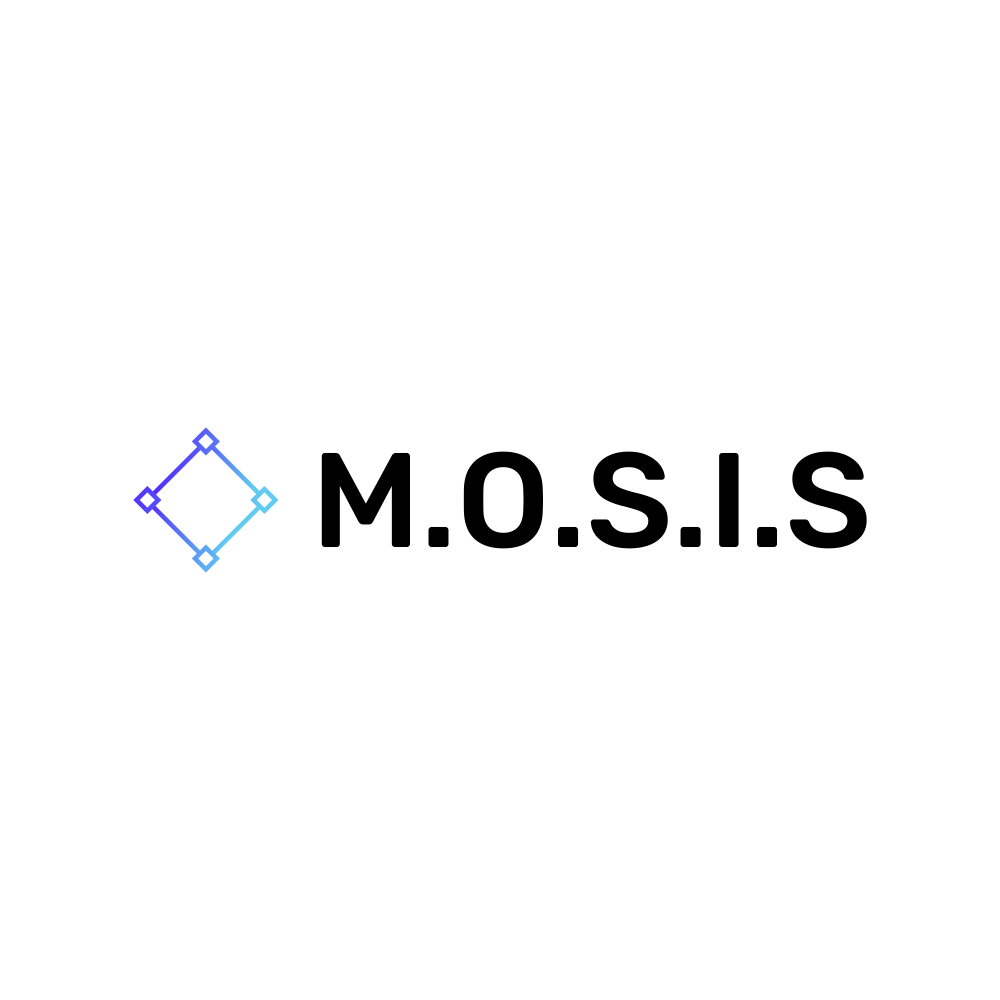
\includegraphics[scale=0.2]{../Title_Page/default.png}\\
    \Huge{\underline{M.O.S.I.S Host Software}\\}
    \Huge{\underline{User Guide}\\}
    \vspace{5cm}
    \large by\\
    Fabio J. Matos Nieves\\
    \normalsize
  \end{center}
\end{titlepage}

\tableofcontents
\newpage
\section{New Features}
\subsection{App}
\begin{itemize}
\item Database schema representation in SQLAlchemy
\item Insertion Statements for MediaEntry and MediaMetadata using SQLAlchemy ORM
\item Type enforcement when inserting into and reading from database.
\item Templated front page and media entry pages
\item Automatic front page generation from database.
\item Solidified MediaEntry title format
\item Random: image, pH, temperature, pressure, dissolved oxygen, shot type, illumination type, ISO, aperture size, shutter speed, white balance, MediaEntry and MediaMetaData generators.
 \item  
\end{itemize}
\subsection{Test Data Generator}
\section{Usage}
\appendix
\section{Host Software Architecture}
\begin{figure}[H]
  \resizebox{\textwidth}{!}{
  \import{./Figures}{class_diagram}
  }
  \caption{M.O.S.I.S Host Software Class Diagram}
\end{figure}
\begin{figure}[H]
  \resizebox{\textwidth}{!}{
  \import{./Figures}{ER_diagram}
  }
  \caption{M.O.S.I.S Host Software Entity Relationship Diagram}
\end{figure}
\section{app.py Documentation}
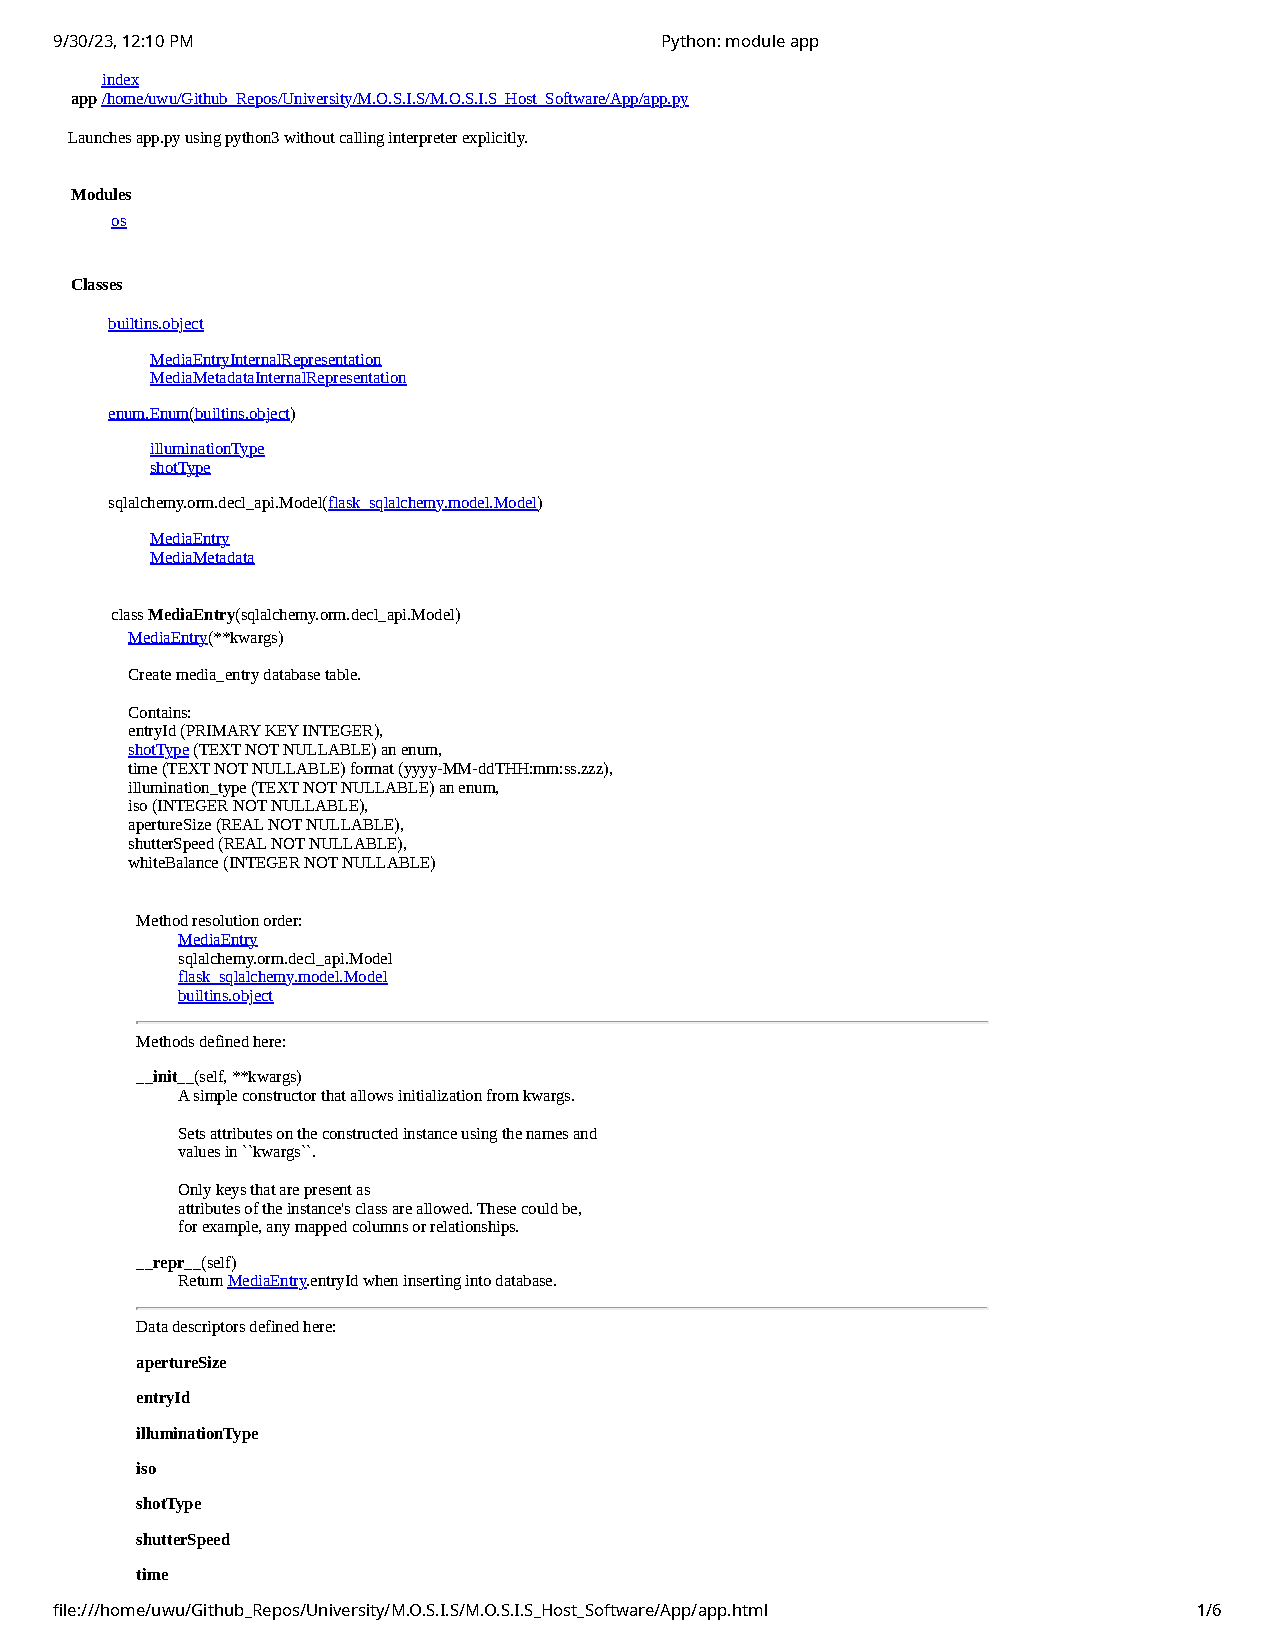
\includepdf[pages=-]{./Figures/app.py_documentation.pdf}
\section{testDataGenerator.py Documenatation}
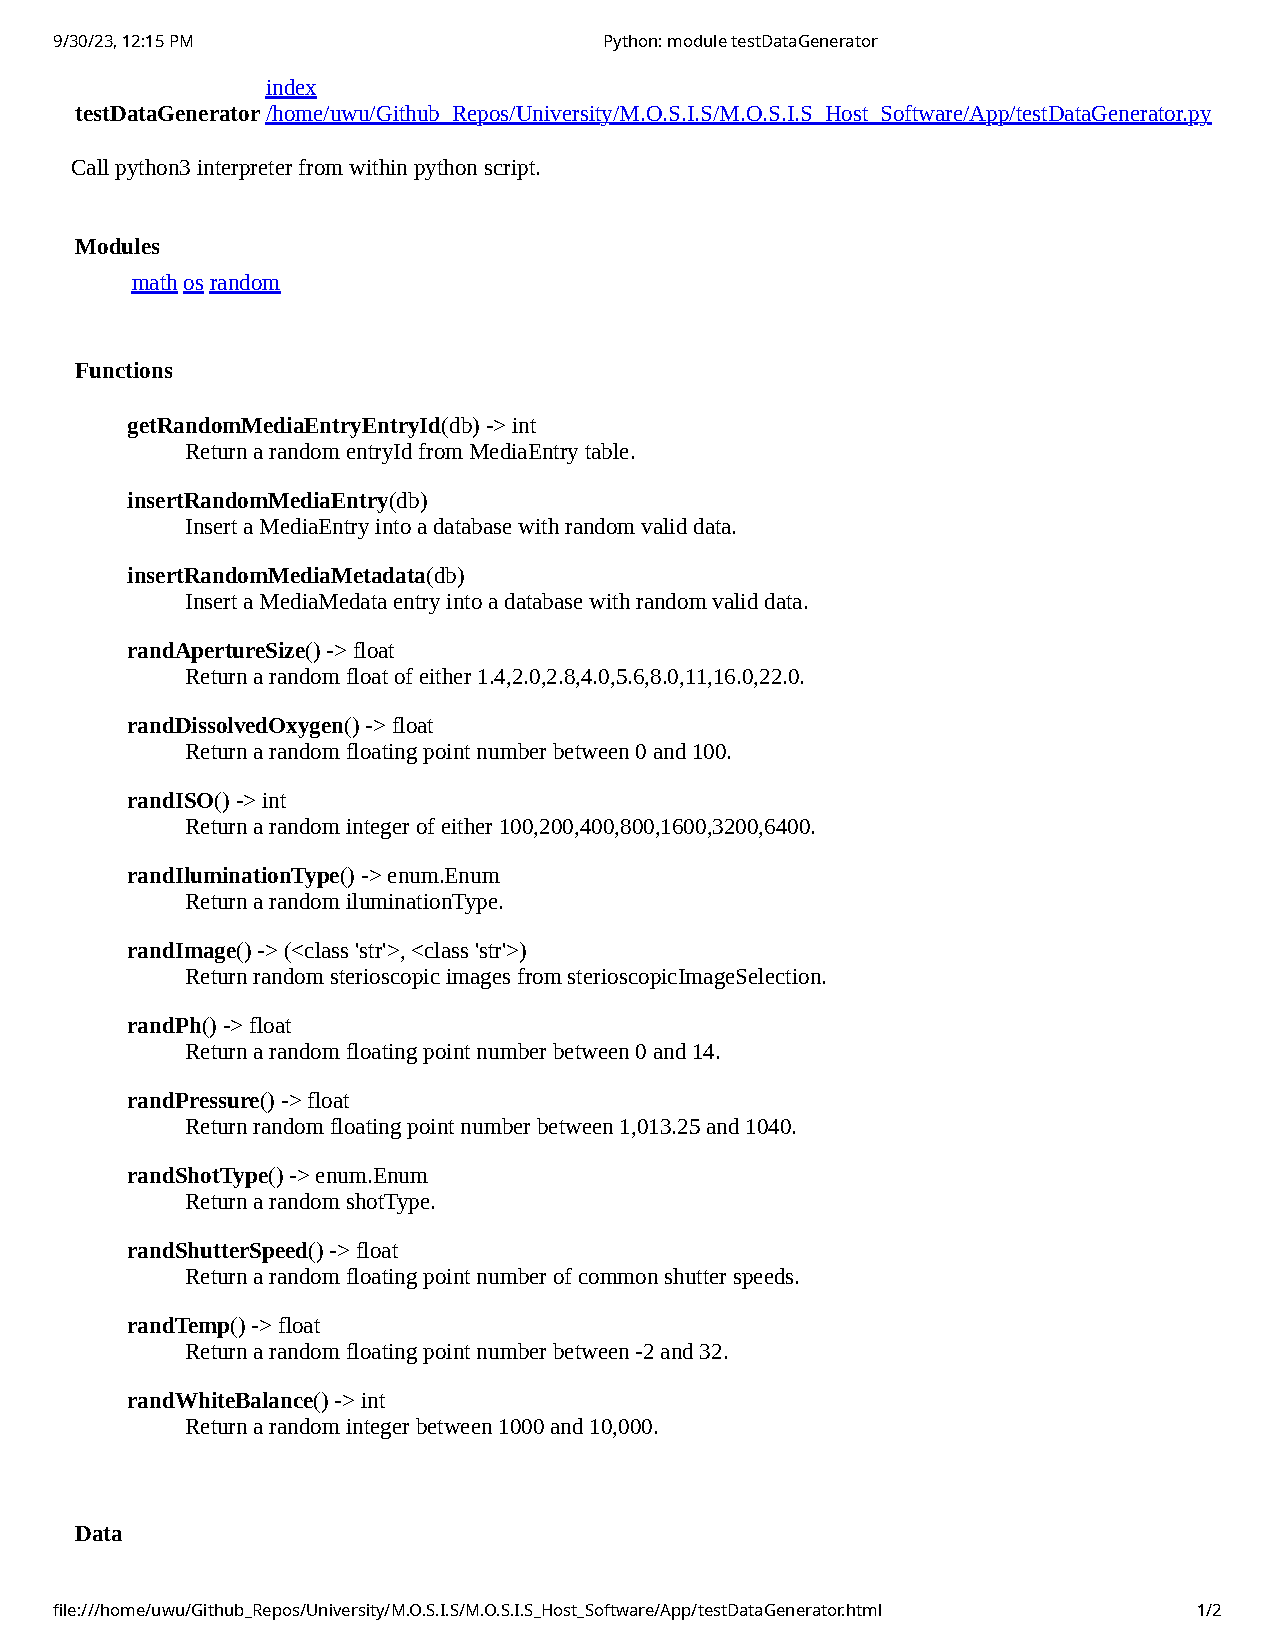
\includepdf[pages=-]{./Figures/testDataGenerator.py_documentation.pdf}
\end{document}